% (angle:distance) :: -360º <= angle <= 720º

\def\upperarrow{
            (sg.north east)+(-0.5,0) arc (0:130:3.8) [rounded corners=0.5]
                -- +(0:0.25) [rounded corners=0.5]
                -- +(-109:0.662) [sharp corners]
                -- +(180:0.65) [rounded corners=0.5]
                -- +(180:0.42) [rounded corners=0.5]
                -- +(180:0.42) arc (132:0:4.3) [rounded corners=0.5]
                -- cycle
              }
              
\def\bottomarrow{
            (d.south west)+(0.5,-0.1) arc (-45:0:-3) [rounded corners=0.5]
                % início seta 1
                -- +(-45:0) arc (0:105:-1) [rounded corners=0.5]
                -- +(100:0.15) [rounded corners=0.5]
                -- +(15:0.4) [sharp corners]
                -- +(-70:0.3) [rounded corners=0.5]
                -- +(-70:0.2) [sharp corners]
                -- +(-70:0.2) arc (115:30:-1.1) [sharp corners]
                % fim seta 1
                -- +(0:0) arc (30:90:-1.5) [rounded corners=0.5]
                % início seta 2
                -- +(0:0) arc (91:109:-7.5) [rounded corners=0.5]
                -- +(100:0.15) [rounded corners=0.5]
                -- +(15:0.4) [sharp corners]
                -- +(-70:0.3) [rounded corners=0.5]
                -- +(-70:0.2) [sharp corners]
                -- +(-70:0.2) arc (109:102:-8.5) [sharp corners]
                % fim seta 2
                % início seta 3
                -- +(0:0) arc (90:110:-10.5) [rounded corners=0.5]
                -- +(100:0.15) [rounded corners=0.5]
                -- +(15:0.4) [sharp corners]
                -- +(-70:0.3) [rounded corners=0.5]
                -- +(-70:0.2) [sharp corners]
                -- +(-70:0.2) arc (115:110:-11.5) [sharp corners]
                % fim seta 3
                % início seta 4
                -- +(0:0) arc (95:108:-11) [rounded corners=0.5]
                -- +(100:0.15) [rounded corners=0.5]
                -- +(15:0.4) [sharp corners]
                -- +(-70:0.3) [rounded corners=0.5]
                -- +(-70:0.2) [sharp corners]
                -- +(-70:0.2) arc (110:90:-12.5) [sharp corners]
                % fim seta 4
                -- +(0:0) arc (90:83:-18.5) [rounded corners=0.5]
                -- +(0:0) arc (83:55:-3) [rounded corners=0.5]
                -- +(0,0) arc (47:35:-2.5) [rounded corners=0.5]
                -- +(0,0) arc (30:-45:-2.5) [rounded corners=0.5]
                -- cycle
            }

\begin{figure}[h!t]{\textwidth}
	\centering
    \caption{definir...} \label{fig:ecredits}
    
    \tikzstyle{arrow} = [thick,->,>=stealth, line width=1pt]
    \tikzstyle{drew} = [draw,fill=white,rounded corners=0.1cm]
    
    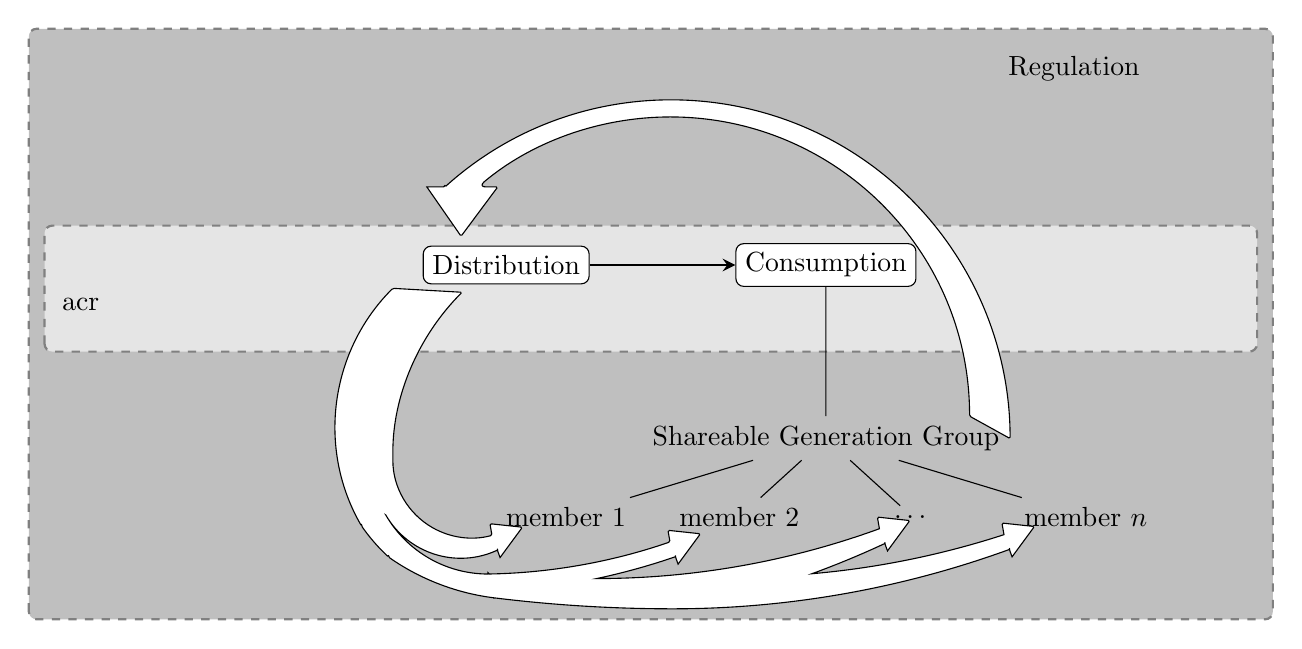
\begin{tikzpicture}[level 1/.style={level distance=2.2cm}, level 2/.style={level distance=1cm, sibling distance=2.2cm}]
        % place dimensions
        \draw[gray,thick,dashed,fill=gray!50,rounded corners=0.1cm] (-2,-6) rectangle (13.8,1.5);
        \draw[gray,thick,dashed,fill=gray!20,rounded corners=0.1cm] (-1.8,-2.6) rectangle (13.6,-1);
        
        % place nodes
        \node[anchor=west, text width=10em]	at (-1.7, -2)	(o) {\gls{acr}};
        \path (o.east)+(2,0.5) node[drew] (d) {Distribution};
		\path (d.east)+(3,0) node[drew] (c) {Consumption}
		    child { node (sg) {Shareable Generation Group}
		        child { node (m1) {member 1} }
		        child { node {member 2} }
		        child { node {\dots} }
		        child { node {member $n$} }
	       % \foreach \k in {1,...,10}{
	       %     child { node {member \k} }
	       % } % dá errado 
	        };
        \path (c.east)+(2,2.5) node		(r) {Regulation};
        
        % draw connections
        \draw[arrow] (d) -- (c);
        \draw[drew] \upperarrow;
        \draw[drew] \bottomarrow;
        
    \end{tikzpicture}
    
  	\legend{\textcolor{red}{AINDA ESTÁ ERRADO!} Differences between energy credit distribution among dwellers of a \gls{gd} group.}
    \source{Author.}
\end{figure}